\section{第八周数值分析实验}
\subsection{第一题}
\begin{ex}
	设 $f(x)=\frac{1}{1+x^2}$, 在 $[-5,5]$ 上分别利用 $T_{11}(x), T_{15}(x), T_{21}(x)$ 的零点作为插值点,构造 $10$ 次, $14$ 次, $20 $次插值多项式 $L_{10}(x), L_{14}(x), L_{20}(x)$, 并作图表示; 此外, 作出误差曲线 $f(x)-L_{10}(x), f(x)-L_{14}(x), f(x)-L_{20}(x)$.
\end{ex}
\lstinputlisting[language=matlab]{day7/chebyshev.m}
%\begin{figure}[H]
%	\centering
%	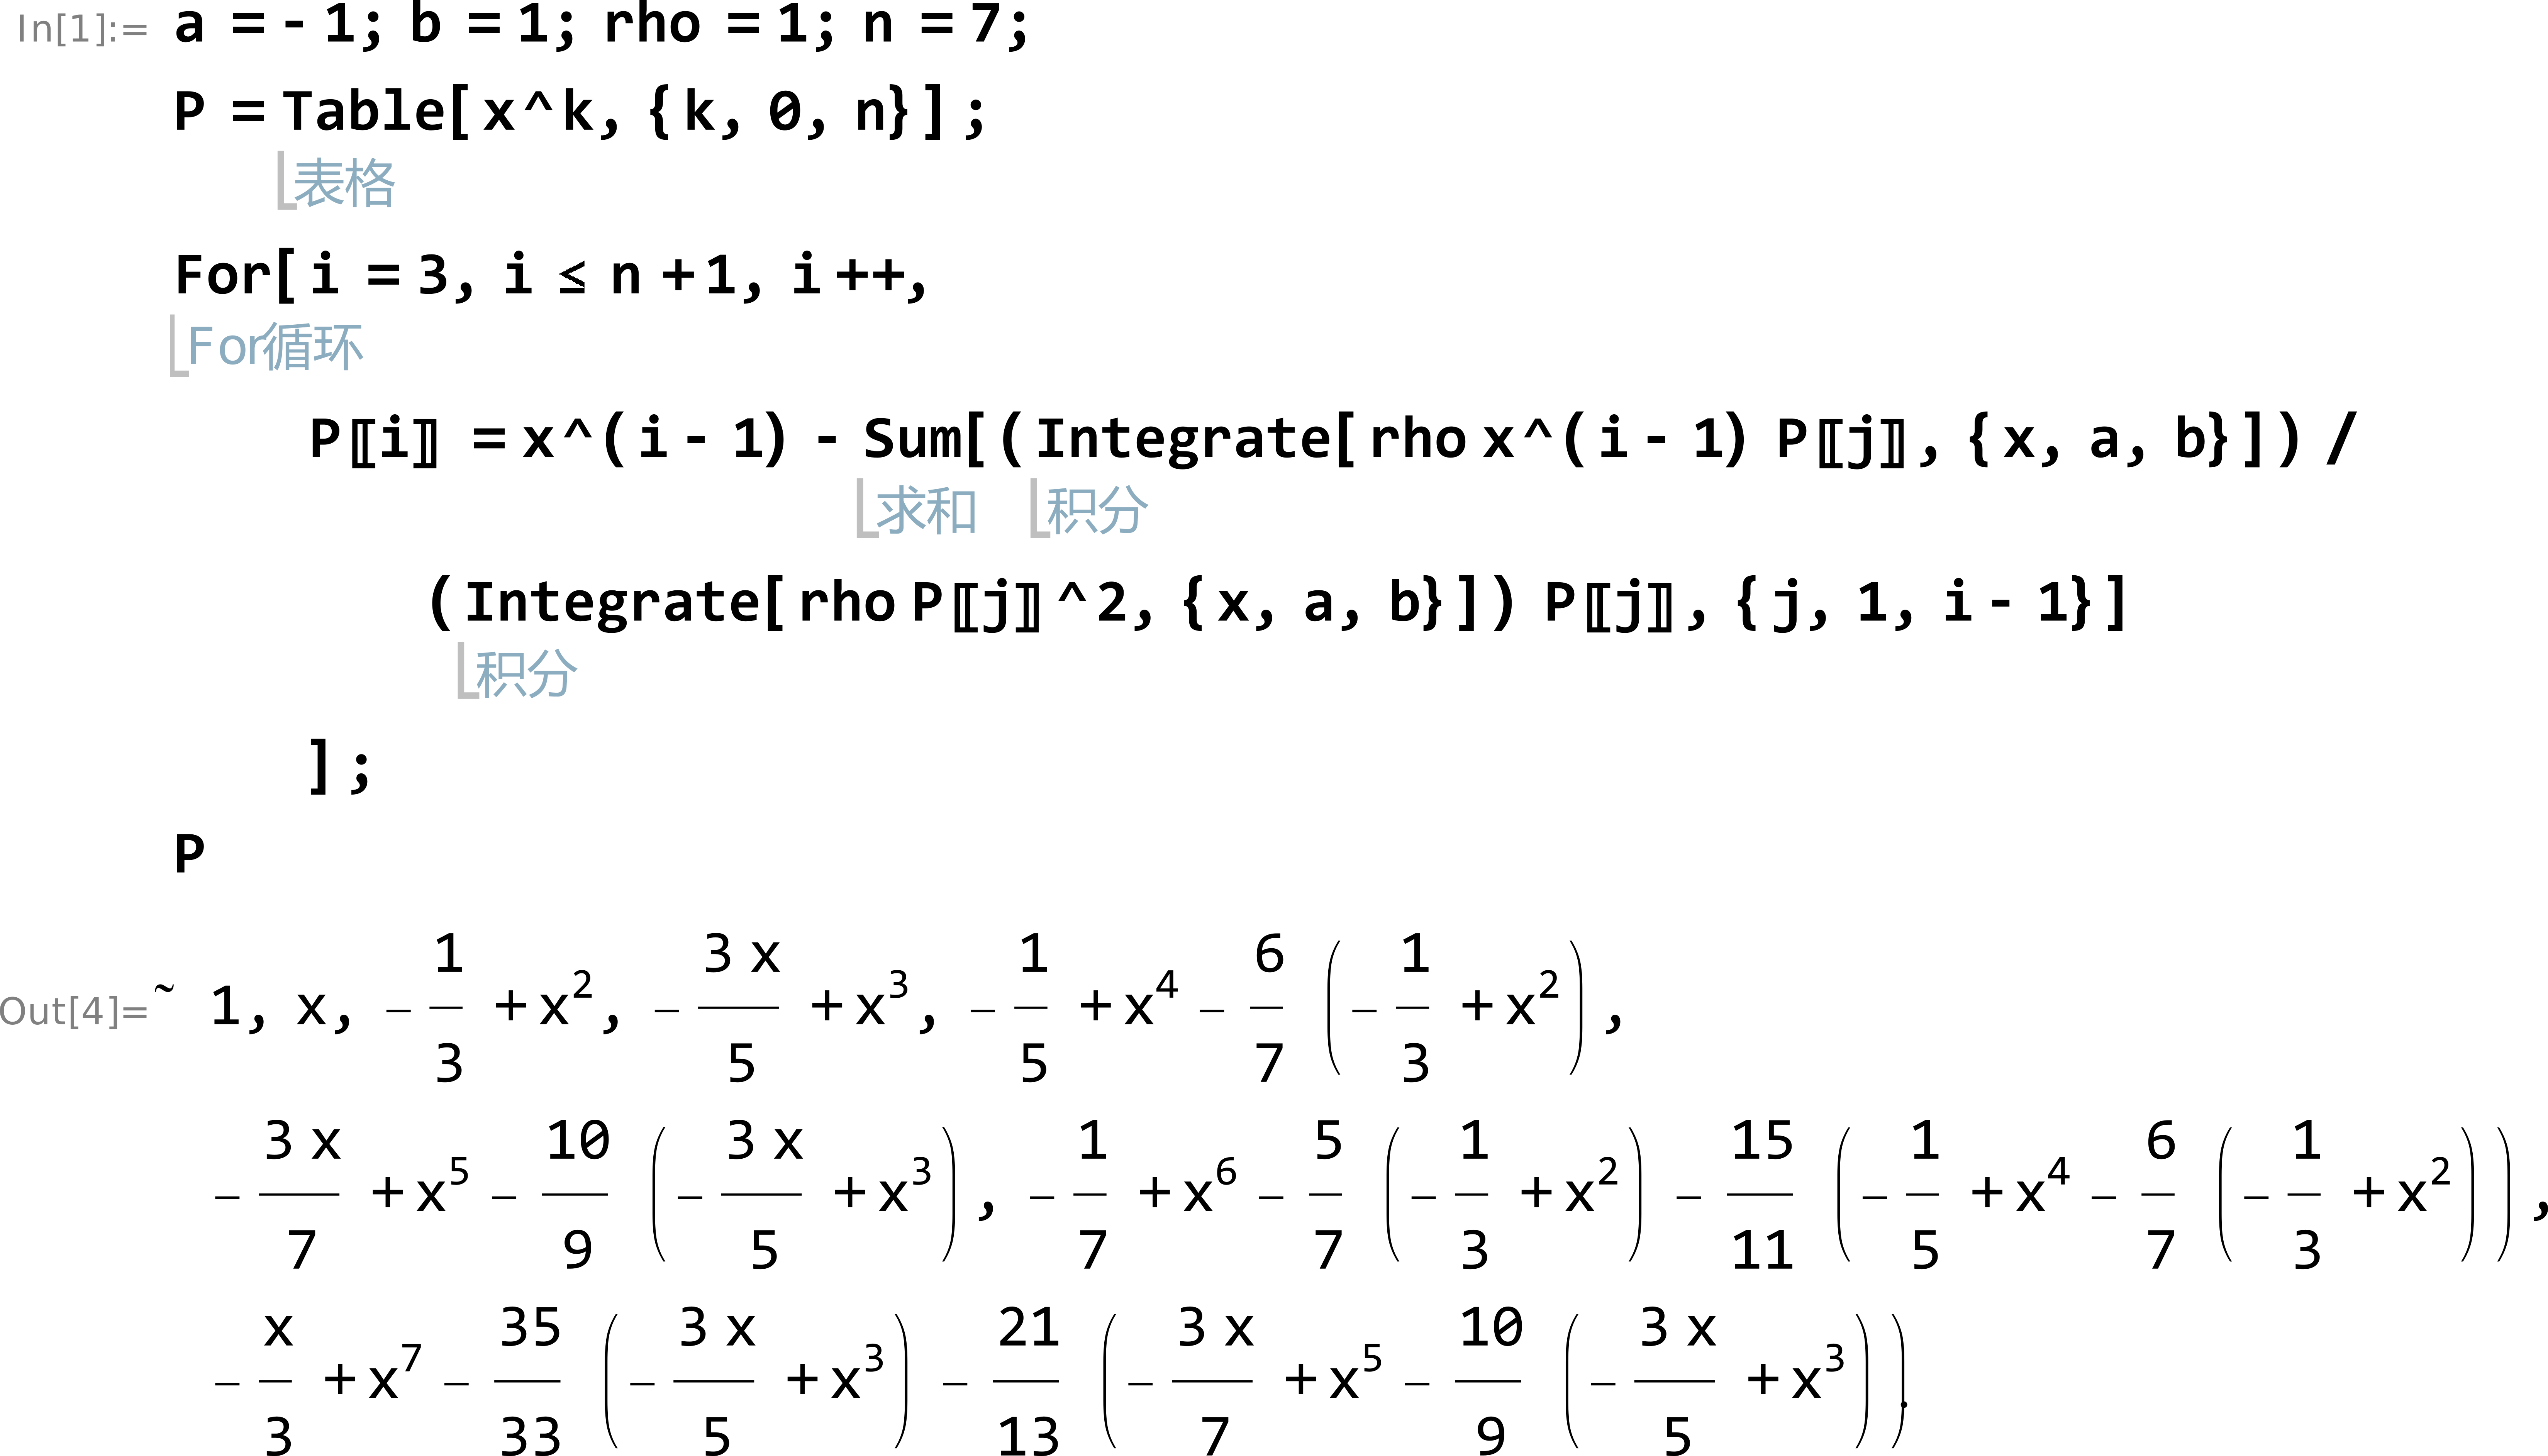
\includegraphics[width = 1\linewidth]{day6/fig1.png}
%	\caption{图示}
%\end{figure}
\begin{figure}[H]
	\centering
	\subfloat[Lagrange插值多项式图像]{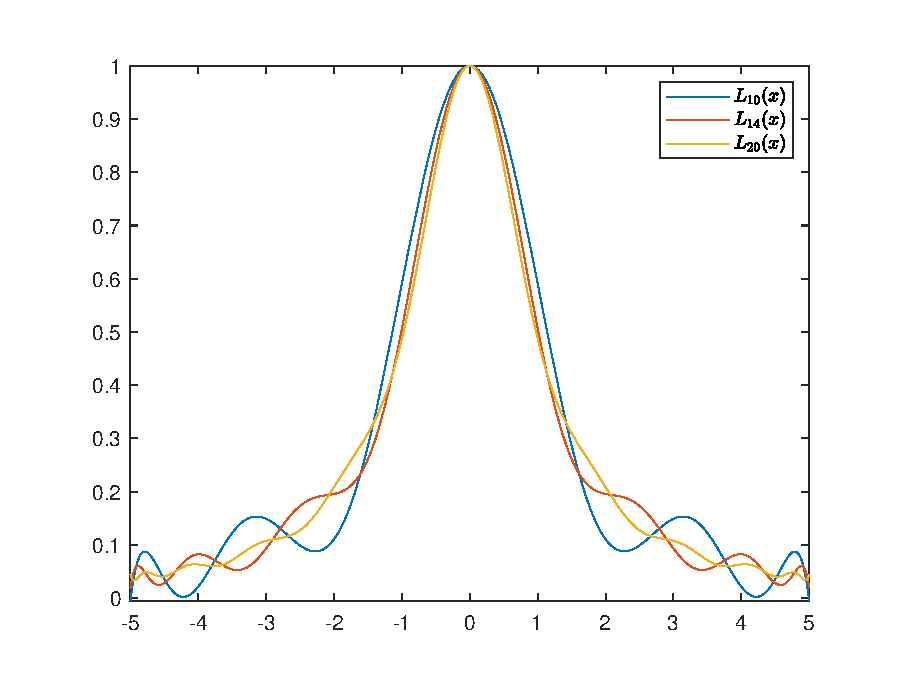
\includegraphics[width = 0.5\linewidth]{day7/q1fig1.eps}}
	\hfill
	\subfloat[误差曲线$f(x)-L_n(x)$]{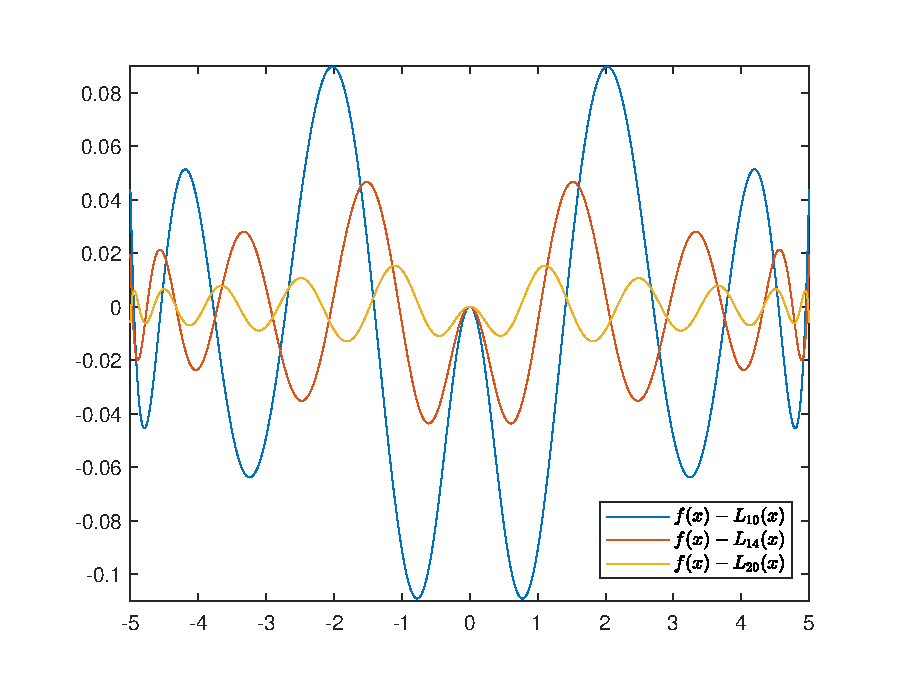
\includegraphics[width = 0.5\linewidth]{day7/q1fig2.eps}}
	\caption{结果图示}
\end{figure}
\subsection{第二题}
\begin{ex}
	设 $f(x)=2 x^4-3 x^3+2 x-1$, 绘制 $[0,1]$ 上的三次最佳一致逼近多项式 $P_3(x)$,二次最佳平方逼近多项式 $S_2(x)$, 伯恩斯坦多项式 $B_1(f, x), B_2(f, x), B_3(f, x)$.
\end{ex}
\lstinputlisting[language=matlab]{day7/q2.m}
\begin{figure}[H]
	\centering
	\subfloat[Berstein多项式及$P_3(x)$图像]{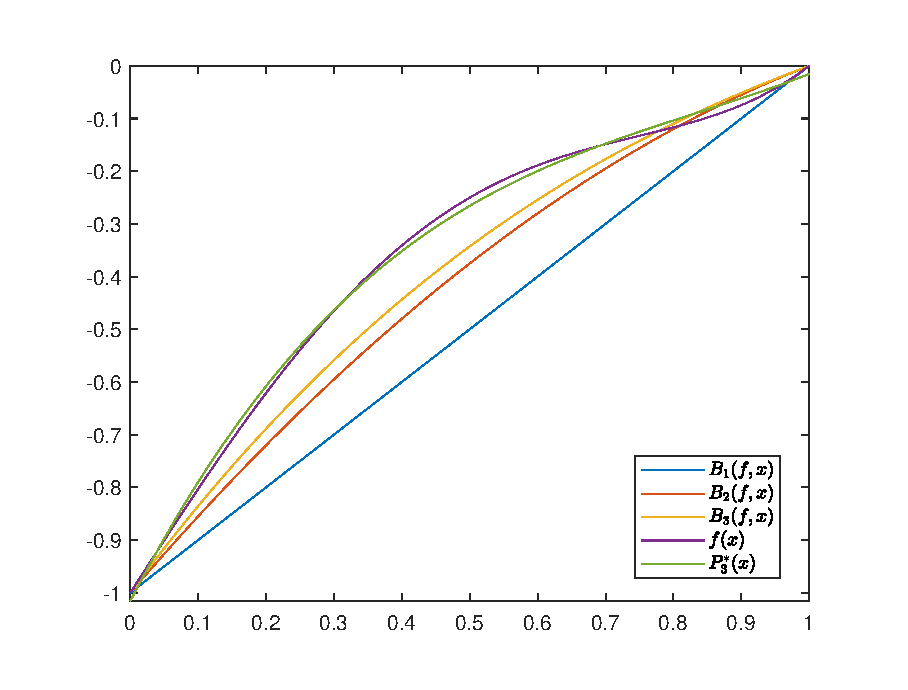
\includegraphics[width = 0.5\linewidth]{day7/q2fig1.eps}}
	\hfill
	\subfloat[二次最佳平方逼近$S_2(x)$]{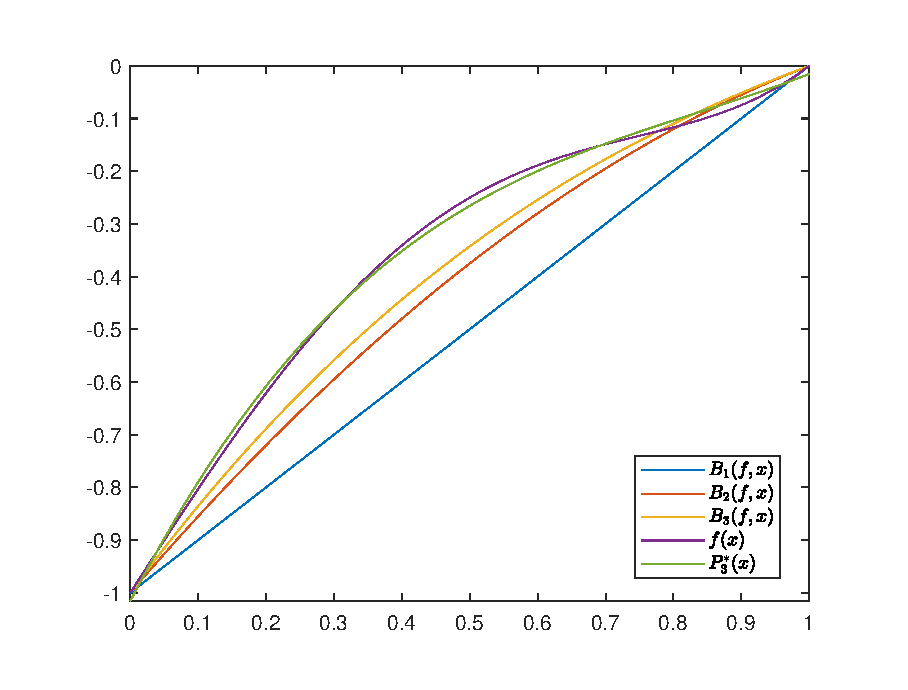
\includegraphics[width = 0.5\linewidth]{day7/q2fig1.eps}}
	\caption{结果图示}
\end{figure}